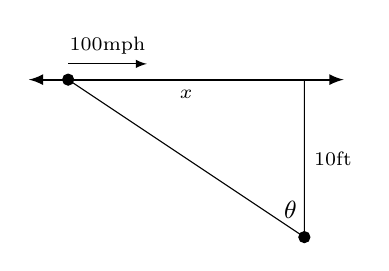
\begin{tikzpicture}[>=latex]

\draw (-3,0) -- (0,0) -- (0,-2) node [shift={(-5pt,10pt)}] {\small $\theta$} node [right,pos=.5] {\scriptsize 10ft}-- cycle;
\draw [<->, thick] (-3.5,0) -- node [below,pos=.5] {\scriptsize $x$} (.5,0);
\draw [fill={\colortwo},draw={\colortwo}] (-3,0) circle (2pt);
\draw [fill=black] (0,-2) circle (2pt);
\draw [->] (-3,.2) -- (-2,.2) node [above,pos=.5] {\scriptsize 100mph};

\end{tikzpicture}
